\chapter{Introduzione alla compatibilità elettromagnetica}
I dispositivi e i sistemi elettrici ed elettronici sono intrinsecamente caratterizzati dall'emissione intenzionale o spuria di segnali elettromagnetici. La Compatibilità Elettromagnetica (EMC) studia la capacità di un dispositivo o apparato di funzionare in modo soddisfacente nel proprio ambiente operativo, senza introdurre disturbi elettromagnetici intollerabili verso altri apparati presenti nello stesso ambiente e garantendo una adeguata robustezza alle interferenze esterne.
\begin{figure}[H]
	\centering
	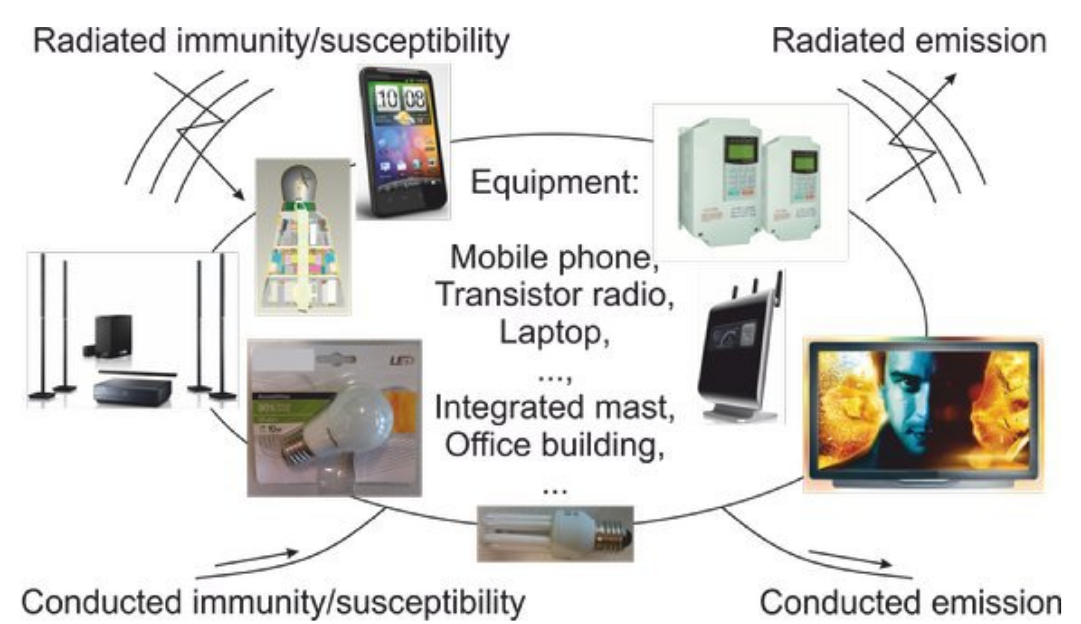
\includegraphics[width=0.5\linewidth]{immagini/introduzione1}
\end{figure}
Si definiscono i termini fondamentali della disciplina:
\begin{itemize}
    \item \textbf{EUT (Equipment Under Test)} $\rightarrow$ apparato, dispositivo o sottosistema sottoposto a prove di verifica, misura e qualificazione di laboratorio per certificarne la conformità alle norme.
    \item \textbf{Emissione} $\rightarrow$ fenomeno per cui un EUT genera e disperde energia elettromagnetica nell'ambiente circostante; si suddivide in \textbf{emissioni condotte} (propagate lungo linee di alimentazione o cavi di segnale) ed \textbf{emissioni irradiate} (propagate nello spazio libero sotto forma di campi elettromagnetici).
    \begin{figure}[H]
    	\centering
    	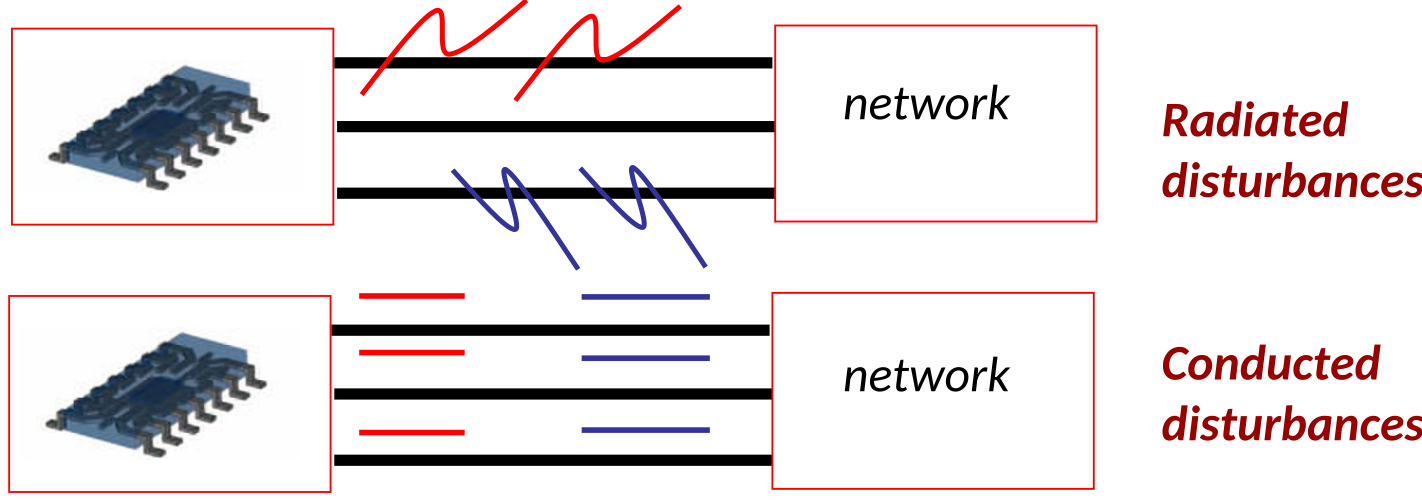
\includegraphics[width=0.5\linewidth]{immagini/introduzione2}
    \end{figure}
    \item \textbf{Immunità} $\rightarrow$ grado di robustezza intrinseca di un apparato che gli consente di mantenere inalterate le prestazioni operative attese in presenza di disturbi elettromagnetici esterni condotti o irradiati.
    \item \textbf{Suscettibilità} $\rightarrow$ vulnerabilità o sensibilità delle prestazioni dell'EUT al degrado funzionale, malfunzionamento logico o danno permanente quando investito da un disturbo elettromagnetico esterno (grandezza opposta all'immunità).
\end{itemize}

Perché un prodotto elettronico possa essere ritenuto conforme e commercializzabile, la progettazione deve soddisfare simultaneamente tre requisiti cogenti:
\begin{itemize}
    \item Limitazione dei livelli di emissione elettromagnetica (condotta e irradiata) generati verso l'ambiente esterno al di sotto delle soglie massime imposte dalle norme tecniche.
    \item Conseguimento di un grado soddisfacente di immunità rispetto alle perturbazioni elettromagnetiche attese nell'ambiente di funzionamento (campi irradiati, transitori condotti, scariche elettrostatiche).
    \item Mantenimento della compatibilità interna tra i singoli sottosistemi compresenti all'interno del medesimo involucro (ad esempio tra alimentatore a commutazione, microcontrollore e ricetrasmettitore RF).
\end{itemize}

Il soddisfacimento dei requisiti EMC costituisce un vincolo di legge obbligatorio per l'accesso ai mercati commerciali:
\begin{itemize}
    \item \textbf{Mercato Europeo (Marchio CE)} $\rightarrow$ la Direttiva Comunitaria Europea 89/336 e le sue successive evoluzioni regolamentari stabiliscono i requisiti essenziali di protezione EMC la cui conformità è prerequisito obbligatorio per l'affissione della Marcatura CE e la vendita negli Stati membri.
    \item \textbf{Mercato Statunitense (Normativa FCC)} $\rightarrow$ la Federal Communications Commission (FCC) disciplina le emissioni mediante le prescrizioni FCC Part 15, distinguendo rigorosamente tra Classe A (dispositivi commerciali, industriali e aziendali) e Classe B (dispositivi per ambienti domestici e residenziali, soggetti a limiti di emissione notevolmente più restrittivi).
\end{itemize}
\begin{figure}[H]
	\centering
	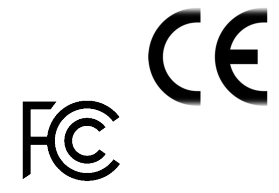
\includegraphics[width=0.2\linewidth]{immagini/introduzione3}
\end{figure}

Ci sono due metodi di analisi fondamentali nel mondo della compatibilità elettromagnetica: tool di \textbf{simulazione} e \textbf{misure} vere e proprie \textbf{in camera anecoica}.
\begin{figure}[H]
	\centering
	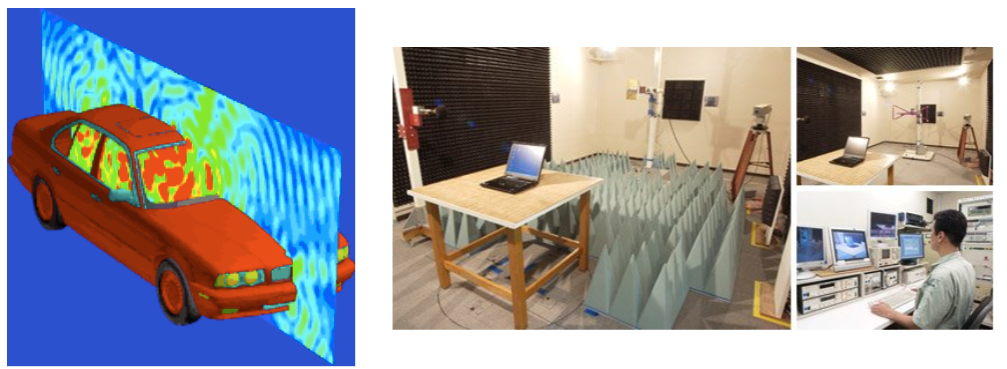
\includegraphics[width=0.7\linewidth]{immagini/introduzione4}
\end{figure}
Ad oggi, in alcuni ambiti, è sufficiente l'ambiente simulativo per ottenere una certificazione vista l'accuratezza raggiunta da questi tools. Possiamo infatti osservare nei diagrammi di flusso della produzione di un dispositivo, distinguendo tra \textbf{approccio tradizionale e moderno}, che la parte di simulazione non è più relegata solo alla fase di design del dispositivo, ma anche a molte altre fasi.
\begin{figure}[H]
	\centering
	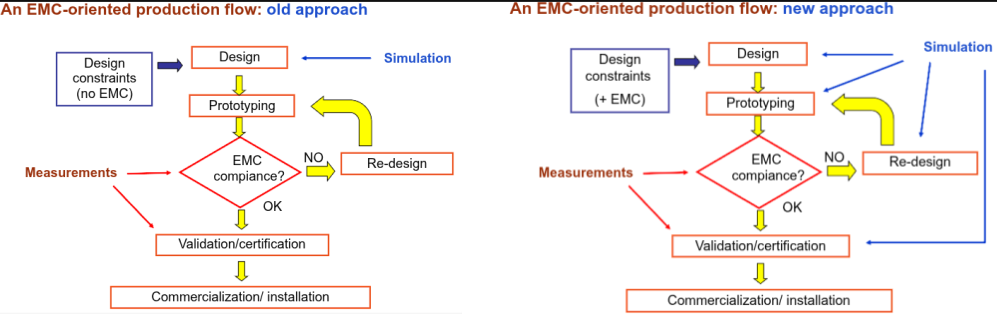
\includegraphics[width=1\linewidth]{immagini/introduzione5}
\end{figure}

La progressiva evoluzione tecnologica dei circuiti integrati ha accentuato la vulnerabilità dei sistemi elettronici ai fenomeni di interferenza, principalmente a causa di tre fattori:
\begin{itemize}
    \item \textbf{Incremento delle frequenze di lavoro} $\rightarrow$ l'innalzamento delle frequenze di clock e di commutazione da decine di $\text{kHz}$ a molti $\text{GHz}$ determina una riduzione della lunghezza d'onda associata ($\lambda$) fino all'ordine di grandezza dei centimetri o millimetri.
    \item \textbf{Riduzione delle tensioni di alimentazione} $\rightarrow$ la transizione dai livelli logici tradizionali a $5.0\,\text{V}$ verso valori pari a $3.3\,\text{V}$, $1.8\,\text{V}$, $1.0\,\text{V}$ e inferiori riduce sensibilmente il margine di rumore logico, rendendo critici disturbi parassiti dell'ordine dei decimi di volt un tempo ininfluenti.
    \item \textbf{Comportamento distribuito delle piste PCB} $\rightarrow$ quando la frequenza aumenta, piste conduttive lunghe pochi centimetri diventano comparabili a un quarto della lunghezza d'onda ($\lambda/4$) di armoniche veloci o disturbi esterni (segnali radiomobili GSM, LTE, emissioni radar), comportandosi come antenne risonanti ad alta efficienza di captazione ed irraggiamento.
\end{itemize}

In merito all'interazione tra campi elettromagnetici a radiofrequenza e salute umana, la letteratura scientifica accertata e le organizzazioni sanitarie internazionali (ICNIRP, OMS) riconoscono unicamente effetti di natura termica, derivanti dal riscaldamento dei tessuti per assorbimento di energia elettromagnetica. La grandezza fisica impiegata per normare e limitare l'esposizione è:
\begin{itemize}
    \item \textbf{SAR (Specific Absorption Rate)} $\rightarrow$ tasso di assorbimento specifico, espresso in $\text{W/kg}$, che quantifica la potenza elettromagnetica assorbita per unità di massa corporea.
\end{itemize}
Rigorosi test sperimentali condotti secondo protocolli in doppio cieco con uso di placebo hanno attestato l'assenza di nessi causali tra la presenza effettiva del campo elettromagnetico e sintomi di ipersensibilità elettromagnetica, confermando che gli attuali limiti di legge, calibrati per scongiurare il surriscaldamento tissutale, garantiscono adeguati margini di sicurezza.

\section{Modello tripartito e meccanismi fisici di accoppiamento}
Qualsiasi fenomeno di interferenza elettromagnetica può essere formalizzato e analizzato attraverso un modello tripartito costituito da tre elementi sequenziali:
\begin{itemize}
    \item \textbf{Sorgente} $\rightarrow$ circuito, dispositivo o sorgente naturale che origina la perturbazione elettrica o magnetica.
    \item \textbf{Percorso di accoppiamento} $\rightarrow$ mezzo fisico o geometrico attraverso il quale l'energia elettromagnetica si propaga dalla sorgente alla vittima.
    \item \textbf{Ricevitore} $\rightarrow$ dispositivo, terminazione circuitale, linea sensibile o tessuto biologico che subisce il disturbo e manifesta un'alterazione funzionale o di prestazione.
\end{itemize}
\begin{figure}[H]
	\centering
	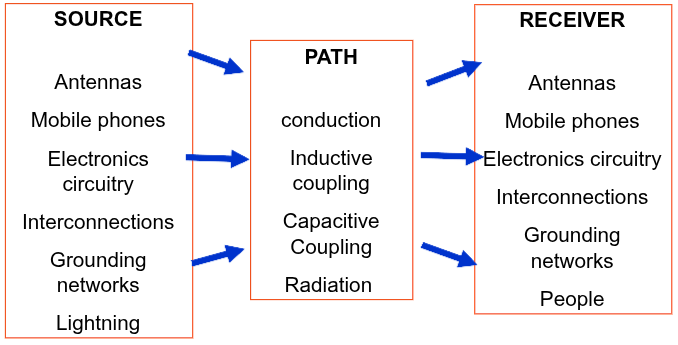
\includegraphics[width=0.7\linewidth]{immagini/introduzione6}
\end{figure}

I percorsi e i meccanismi di accoppiamento guidano fortemente le scelte progettuali e determinano le contromisure da implementare. 
\begin{figure}[H]
	\centering
	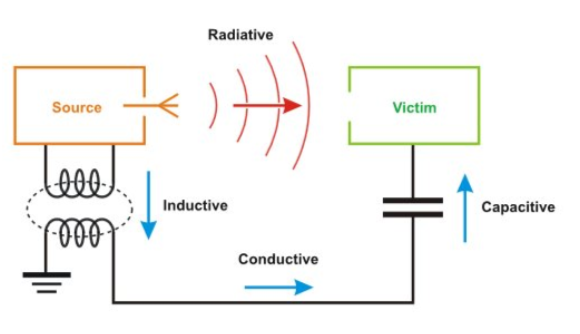
\includegraphics[width=0.7\linewidth]{immagini/introduzione7}
\end{figure}
Nel fenomeno del \textbf{crosstalk} tra conduttori (cavo aggressore e cavo vittima):
\begin{itemize}
	\item \textbf{Accoppiamento capacitivo} $\rightarrow$ il segnale impulsivo sull'aggressore si trasferisce sul cavo vittima tramite campo elettrico. La possibile soluzione è l'uso di \textbf{cavi schermati (shielded cables)}.
	\item \textbf{Accoppiamento induttivo} $\rightarrow$ la commutazione di corrente sull'aggressore induce transienti sul cavo vittima tramite campo magnetico. La possibile soluzione è l'uso di \textbf{cavi intrecciati (twisted cables)}.
\end{itemize}
\begin{figure}[H]
	\centering
	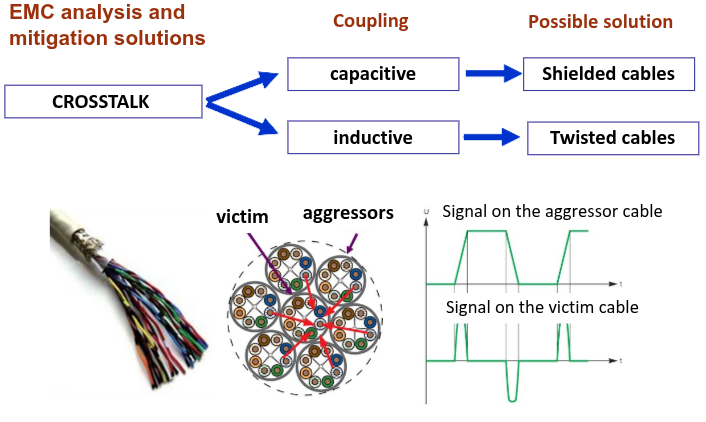
\includegraphics[width=0.7\linewidth]{immagini/introduzione8}
\end{figure}

Per quanto concerne i fenomeni di \textbf{emissione}:
\begin{itemize}
	\item \textbf{Accoppiamento conduttivo} $\rightarrow$ il disturbo si propaga per conduzione lungo i conduttori. La possibile soluzione è il \textbf{filtraggio (filtering)}.
	\item \textbf{Accoppiamento radiativo} $\rightarrow$ il disturbo si propaga per irraggiamento nello spazio libero. La possibile soluzione è la \textbf{schermatura (shielding)}.
\end{itemize}
\begin{figure}[H]
	\centering
	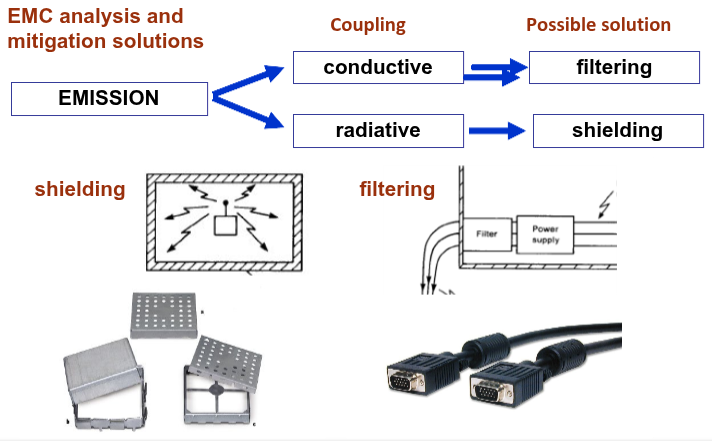
\includegraphics[width=0.7\linewidth]{immagini/introduzione9}
\end{figure}

\section{Metodologie di misura e prove di laboratorio EMC}
\begin{figure}[H]
	\centering
	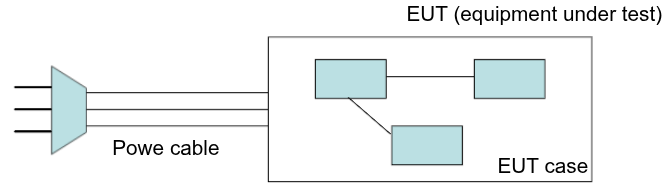
\includegraphics[width=0.7\linewidth]{immagini/introduzione10}
\end{figure}
Le principali prove sperimentali condotte sull'EUT (alimentato tramite il proprio cavo di alimentazione e racchiuso nel proprio involucro) si suddividono in due categorie:
\newpage
\begin{itemize}
	\item \textbf{Prove di emissione}:
	\begin{itemize}
		\item Emissioni irradiate.
		\item Emissioni condotte.
		\item Emissione di correnti armoniche.
		\item Emissione di disturbi dall'alimentazione.
	\end{itemize}
	\item \textbf{Prove di immunità}:
	\begin{itemize}
		\item Campi elettromagnetici irradiati.
		\item Campi elettromagnetici condotti.
		\item Scariche elettrostatiche (ESD).
		\item Transitori veloci (EFT/BURST).
		\item Sovratensioni e buchi di tensione.
	\end{itemize}
\end{itemize}

La stesura dei requisiti tecnici sono demandate a comitati normativi dedicati:
\begin{itemize}
	\item \textbf{IEC} (International Electrotechnical Commission) $\rightarrow$ comitato normativo internazionale responsabile degli standard elettrotecnici generali.
	\item \textbf{CISPR} (Comité International Spécial des Perturbations Radioélectriques) $\rightarrow$ comitato internazionale specializzato nella definizione delle metodologie e dei limiti di misura delle interferenze radio.
	\item \textbf{CENELEC} (Comité Européen de Normalisation Électrotechnique) $\rightarrow$ organismo di armonizzazione normativa dell'Unione Europea per il settore elettrotecnico.
	\item \textbf{CEI} (Comitato Elettrotecnico Italiano) $\rightarrow$ ente normatore nazionale italiano, all'interno del quale il Comitato Tecnico CT 210 si occupa della standardizzazione della compatibilità elettromagnetica.
\end{itemize}

Le misure di emissione sono normate in bande di frequenza dedicate:
\begin{itemize}
	\item \textbf{Emissioni condotte} $\rightarrow$ banda di frequenza compresa tra $150\,\text{kHz}$ e $30\,\text{MHz}$.
	\item \textbf{Emissioni irradiate} $\rightarrow$ banda di frequenza compresa tra $30\,\text{MHz}$ e $1\,\text{GHz}$.
\end{itemize}

I limiti normativi differenziano gli apparati in Classe A e Classe B:
\begin{itemize}
	\item \textbf{Limiti per le emissioni irradiate (misura del campo elettrico a una distanza di $10\,\text{m}$)}:
	\begin{figure}[H]
		\centering
		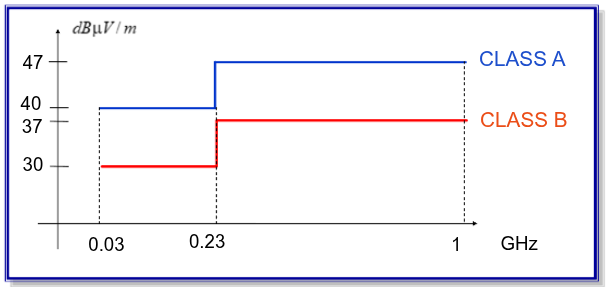
\includegraphics[width=0.5\linewidth]{immagini/introduzione11}
	\end{figure}
	\begin{itemize}
		\item Classe A: limite di $40\,\text{dB}\mu\text{V/m}$ tra $0.03\,\text{GHz}$ ($30\,\text{MHz}$) e $0.23\,\text{GHz}$ ($230\,\text{MHz}$); limite di $47\,\text{dB}\mu\text{V/m}$ tra $0.23\,\text{GHz}$ e $1\,\text{GHz}$.
		\item Classe B: limite di $30\,\text{dB}\mu\text{V/m}$ tra $0.03\,\text{GHz}$ e $0.23\,\text{GHz}$; limite di $37\,\text{dB}\mu\text{V/m}$ tra $0.23\,\text{GHz}$ e $1\,\text{GHz}$.
	\end{itemize}
	\item \textbf{Limiti per le emissioni condotte (tensione di quasi-picco ai pin dell'EUT)}:
	\begin{figure}[H]
		\centering
		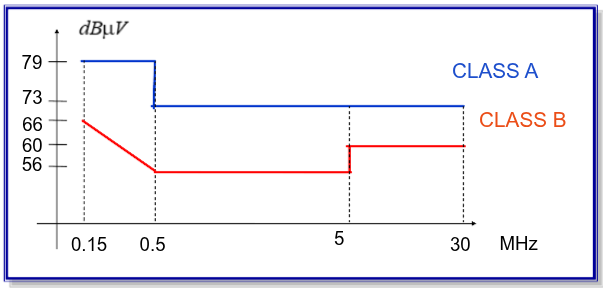
\includegraphics[width=0.5\linewidth]{immagini/introduzione12}
	\end{figure}
	\begin{itemize}
		\item Classe A: limite di $79\,\text{dB}\mu\text{V}$ tra $0.15\,\text{MHz}$ e $0.5\,\text{MHz}$; limite di $73\,\text{dB}\mu\text{V}$ tra $0.5\,\text{MHz}$ e $30\,\text{MHz}$.
		\item Classe B: limite decrescente da $66\,\text{dB}\mu\text{V}$ a $56\,\text{dB}\mu\text{V}$ tra $0.15\,\text{MHz}$ e $0.5\,\text{MHz}$; limite di $56\,\text{dB}\mu\text{V}$ tra $0.5\,\text{MHz}$ e $5\,\text{MHz}$; limite di $60\,\text{dB}\mu\text{V}$ tra $5\,\text{MHz}$ e $30\,\text{MHz}$.
	\end{itemize}
\end{itemize}

Per la caratterizzazione sperimentale delle emissioni e dell'immunità si possono seguire due approcci metodologici:
\begin{enumerate}
	\item \textbf{Approccio Pre-Compliance} $\rightarrow$ impiega strumentazione generica da laboratorio (oscilloscopio digitale, analizzatore di spettro, sonde di tensione e di corrente, sonde di campo vicino). Tale approccio è utilizzato durante le fasi di sviluppo e prototipazione per guidare il design.
	\item \textbf{Approccio Full-Compliance} $\rightarrow$ richiede strumentazione specialistica (ricevitore EMI, rete di stabilizzazione LISN / AMN, reti di accoppiamento/disaccoppiamento CDN, generatori di disturbo), siti di prova dedicati (camera semi-anecoica), setup di misura normalizzati (disposizione dei cavi, lunghezza dei conduttori, posizionamento degli apparati) e procedure di prova standardizzate (impostazioni degli strumenti e metodi di misura). Questo approccio è l'unico valido ai fini dell'ottenimento della marcatura CE, obbligatoria per commercializzare il prodotto nel mercato europeo.
\end{enumerate}

I principali standard internazionali di riferimento studiati per le misure di emissione e per i test di immunità sono le norme EN 55022 ed EN 61000-4-x.

\section{Modellistica EMC}
La modellistica EMC svolge diversi compiti essenziali nell'analisi e nella previsione dei disturbi:
\begin{itemize}
	\item Caratterizzazione delle sorgenti (in particolare delle sorgenti non intenzionali).
	\item Valutazione dei disturbi condotti.
	\item Valutazione dei disturbi irradiati.
	\item Analisi dei transitori elettrici veloci e dei problemi di Signal Integrity.
	\item Analisi della risposta a impulsi di sovratensione (surge pulses).
	\item Modellazione della scarica elettrostatica (ESD).
	\item Valutazione dell'efficacia di schermatura (Shielding Effectiveness).
	\item Valutazione dell'immunità a campi incidenti.
\end{itemize}

\newpage
La formalizzazione di un problema EMC prevede la caratterizzazione interconnessa di tre componenti:
\begin{figure}[H]
	\centering
	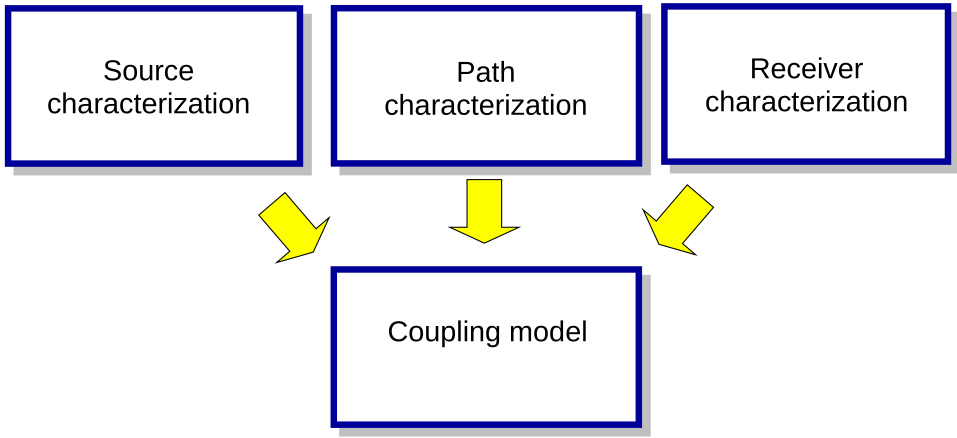
\includegraphics[width=0.6\linewidth]{immagini/introduzione13}
\end{figure}
In linea di principio, qualsiasi problema EMC può essere affrontato risolvendo il modello elettromagnetico completo, formulato mediante le equazioni di Maxwell complete:
\[
\vec{E}, \; \vec{D}, \; \vec{H}, \; \vec{B}, \; \vec{J}, \; \vec{S}, \; \vec{P}
\]
unite alle equazioni costitutive dei materiali e alle condizioni al contorno e iniziali. Tuttavia, tale approccio diventa impraticabile e insostenibile dal punto di vista del calcolo per i casi di interesse pratico: si rende pertanto indispensabile il ricorso a \textbf{modelli semplificati}.

L'approccio generale alla modellazione EMC si articola in quattro passi sequenziali:
\begin{enumerate}
	\item \textbf{STEP 1: Definizione del problema} $\rightarrow$ identificazione di tutte le interazioni elettromagnetiche tra le sottoparti del sistema, sia intenzionali che indesiderate.
	\item \textbf{STEP 2: Segmentazione} $\rightarrow$ scomposizione del sistema complesso e identificazione dei sottosistemi o sottoparti che possono essere modellati in modo indipendente, trattandoli come multi-porte interagenti alle terminazioni.
	\item \textbf{STEP 3: Modellazione dei singoli sottosistemi} $\rightarrow$ scelta del modello elettromagnetico più appropriato (analitico, numerico o sperimentale), caratterizzazione del sottosistema ai suoi terminali e sintesi di un multi-polo equivalente.
	\item \textbf{STEP 4: Simulazione a livello di sistema} $\rightarrow$ risoluzione globale del sistema mediante l'interconnessione dei modelli multi-porta equivalenti sintetizzati per ciascun blocco.
\end{enumerate}

Un esempio applicativo è costituito dallo studio della qualità di un segnale che si propaga lungo un circuito stampato (PCB), configurato come problema di Signal Integrity in presenza di un campo incidente esterno:
\begin{itemize}
	\item \textbf{Definizione del problema}: il sistema comprende uno stadio pilota (driver), una linea di interconnessione (bus), un piano di massa sottostante, uno stadio ricevitore (receiver) e l'interazione con un campo elettromagnetico esterno.
	\begin{figure}[H]
		\centering
		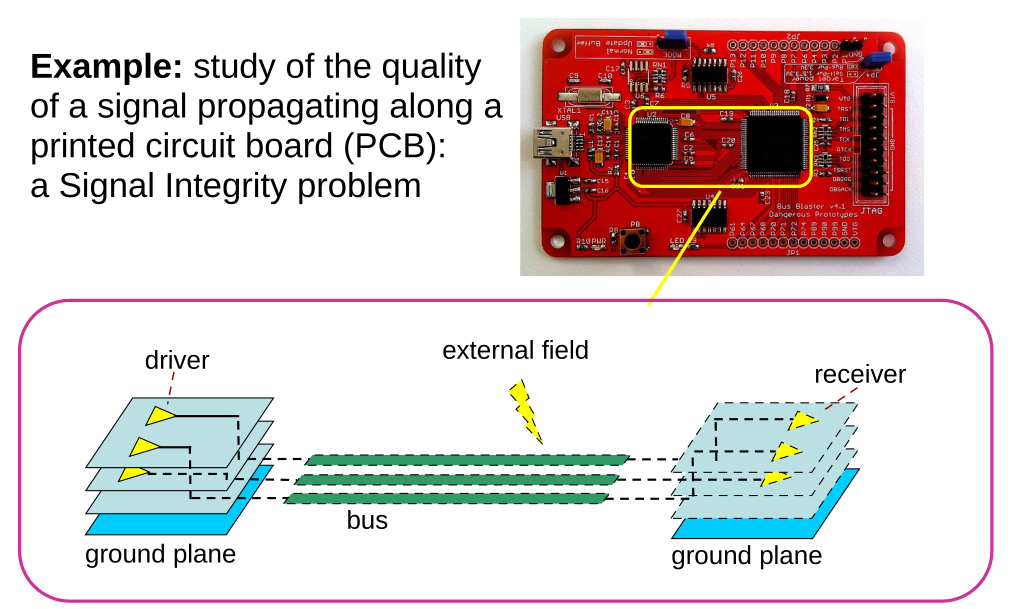
\includegraphics[width=0.55\linewidth]{immagini/introduzione14}
	\end{figure}
	
	\item \textbf{Segmentazione in multi-porte}: il sistema viene scomposto nei seguenti blocchi elementari interagenti alle estremità:
	\begin{itemize}
		\item Blocco Driver.
		\item Blocco linea corta (Short line).
		\item Blocco discontinuità geometrica.
		\item Blocco bus (linea lunga) soggetto all'azione del campo esterno.
		\item Blocco discontinuità geometrica.
		\item Blocco linea corta (Short line).
		\item Blocco ricevitore (Receiver).
	\end{itemize}
	\begin{figure}[H]
		\centering
		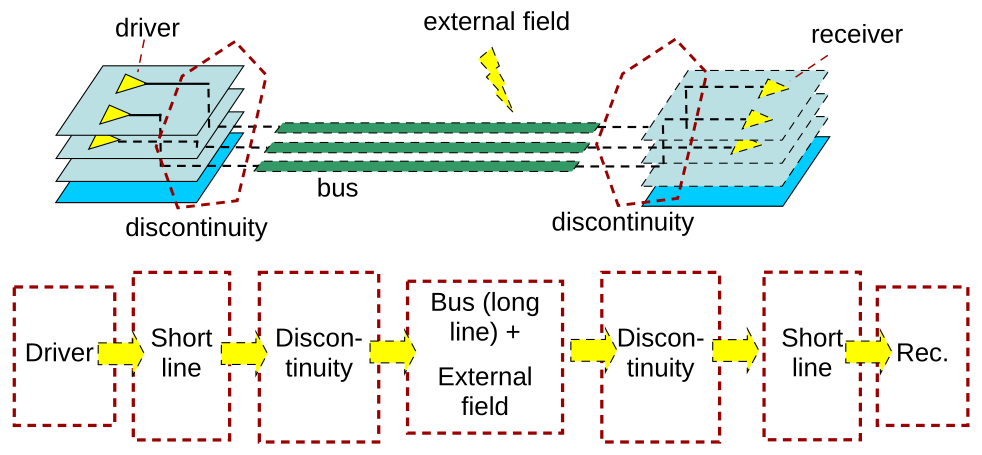
\includegraphics[width=0.55\linewidth]{immagini/introduzione15}
	\end{figure}
	
	\item \textbf{Modellazione e sintesi}: ciascun blocco viene caratterizzato autonomamente ai propri terminali per generare il corrispondente circuito equivalente multi-porta, pronto per la successiva co-simulazione a livello di sistema.
	\begin{figure}[H]
		\centering
		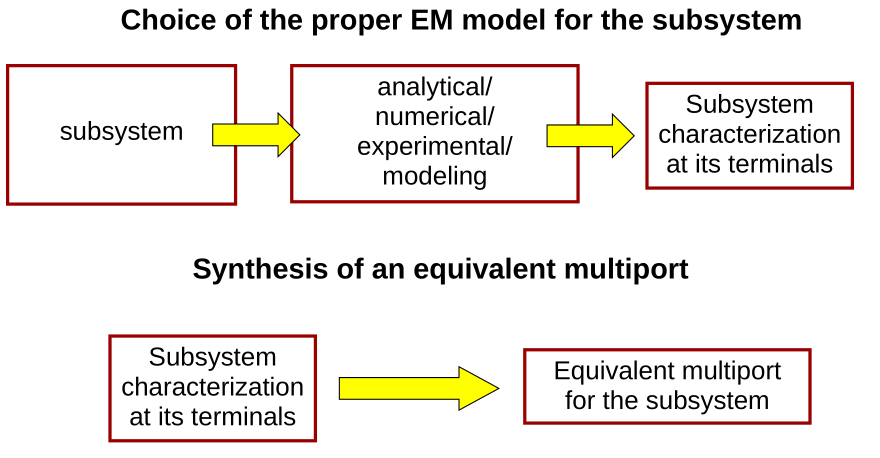
\includegraphics[width=0.6\linewidth]{immagini/introduzione16}
	\end{figure}
\end{itemize}
